\section{任务控制、上下文扩展与证书投递}
\label{sec:delivery}
\subsection{控制完成与验证完成分别建模}
产品的 \code{TaskController} 接受拓扑有序的任务和真实数据依赖，区分 READY、WAITING\_INPUT、BLOCKED、FINISHED 和 FAILED。准备观察、环境预检、工具运行完成、验证器完成、性质证明和整个运行完成是不同事实。验证器合法返回 UNRESOLVED 可以完成协议并解锁依赖，但不提供充分证明。准备成功或 error 不能冒充完成验证器。

可选能力不可用时只阻塞依赖它的任务；独立静态任务继续运行。显式补充输入后重新检查等待及依赖，不凭重试次数猜测前提已满足。无效动作默认最多两次；研究任务图另有显式递归上限 16。受控测试实际执行八个计划任务，并对注入的无进展循环验证有限终止。这些数值约束调度，不证明选中的任务具有高价值。

\begin{figure}[htbp]\centering
\begin{tikzpicture}[node distance=7mm]
\node[smallbox] (ready) {READY};
\node[smallbox,right=12mm of ready] (wait) {WAITING\_INPUT};
\node[smallbox,right=12mm of wait] (blocked) {BLOCKED};
\node[smallbox,below=14mm of ready,fill=green!8] (finished) {FINISHED\\可为 UNKNOWN};
\node[smallbox,below=14mm of wait,fill=warm!8] (failed) {FAILED\\协议 / 内部错误};
\draw[arrow] (ready)--node[above,font=\scriptsize]{缺业务输入}(wait);
\draw[arrow] (wait)--node[above,font=\scriptsize]{依赖不可用}(blocked);
\draw[arrow] (ready)--node[left,font=\scriptsize]{合法返回}(finished);
\draw[arrow] (ready.east)--++(3mm,0)|-node[pos=.8,above,font=\scriptsize]{异常}(failed.west);
\draw[arrow] (wait.north) to[bend right=45] node[above,font=\scriptsize]{显式补充后重检}(ready.north);
\end{tikzpicture}
\caption{任务控制态概念图。状态恢复依赖显式输入和能力检查；性质状态由证据归并另行计算。图展示主要转换，不列出全部实现分支。}
\end{figure}
\loc{application/controller.py; agents/workflow.py; harness/defaults.py}

\subsection{行范围视图与事务性扩展}
\code{SourceReadView} 的授权单位是规范路径和闭区间行号。完整源码清单属于使用者选择的授权根；默认静态索引可内部解析支持文件，但内部解析不是免费模型上下文投递。限定初始范围时，工具只拿到已准入切片。路径相同也不能免费读取另一个行区间。

扩展要求显式 reason、授权清单成员、行范围合法以及重新读取后的字节摘要一致。完整扩展封装按 UTF-8 计费，包含标识、元数据和 JSON 外壳；只有成功投递后才改变视图版本。预算拒绝、源码漂移或越界读取保持原视图。重复投递同一上下文也记账。获准看到 helper 源码之后，仍须建立调用绑定，才能将 helper 语义用于候选证明。

\begin{pseudocode}{alg:context}{先投递、后准入的上下文扩展}
\Pinput{当前视图 $V$、显式 $(p,l_0,l_1,\mathrm{reason})$、授权清单、上下文预算}
\Poutput{更新后的视图与准入回执，或保持原视图的拒绝诊断}
\Pstep{验证规范路径、正行区间、清单成员和明确的扩展理由。}
\Pstep{通过既有安全源码读取边界读取，不跟随符号链接；重核文件字节摘要。}
\Pstep{将请求切片与元数据序列化为完整封装 $s$，计算 $b=|\mathrm{UTF8}(s)|$。}
\Pstep{若 $b$ 超过剩余预算，输出 REJECTED；不改变 $V$。}
\Pstep{成功扣减 $b$ 后将该行区间加入 $V$，计算新的 $H_v$。}
\Pstep{留下 ADMITTED 回执；不改变源码字节身份，也不宣称运行时调用关系已成立。}
\end{pseudocode}
\loc{application/context.py; code_adapters/source_files.py}

\subsection{共享池与最小证书预留}
产品默认观察池 $B=8192$ 字节，独立诊断预留 $D=256$ 字节。\code{allocation_plan} 支持声明各必需证书已验证的最小尺寸 $m_i$；计划可行需满足
\begin{equation}
\sum_i m_i+D\le B.
\end{equation}
一次投递证书 $c_i$ 之前，还须保护其他尚未投递必需证书的预留：
\begin{equation}
|c_i|+\sum_{j\ne i,\,j\notin\mathrm{delivered}}m_j\le B-D-B_{\mathrm{used}}.
\end{equation}
\textbf{当前产品服务没有必须证明成功的义务，实际传入的 \code{minimum_bytes} 是空映射。}预留接口及其正反控制已验收，不应据此声称服务已预测所有语义证明的最小长度。无法投递完整证明时，原结果保留在私有账本，公共 finding 维持 UNKNOWN，运行可形成 PARTIAL。

受控证书反例使用四个完整 JSON 证书，尺寸为 2500、1000、1000、1000 字节。简单平均四分先给第一个任务 2048 字节，短缺 452 字节；共享池在保留 256 字节诊断之后仍可容纳全部 5500 字节，余额 2436 字节。该反例说明平均分配可能拒绝一个总体可行计划，\emph{不证明任意实际工作负载的性能改善}。冻结的研究 E 系列累计均分政策保留，不将产品政策回填为历史实验配置。
\begin{figure}[htbp]\centering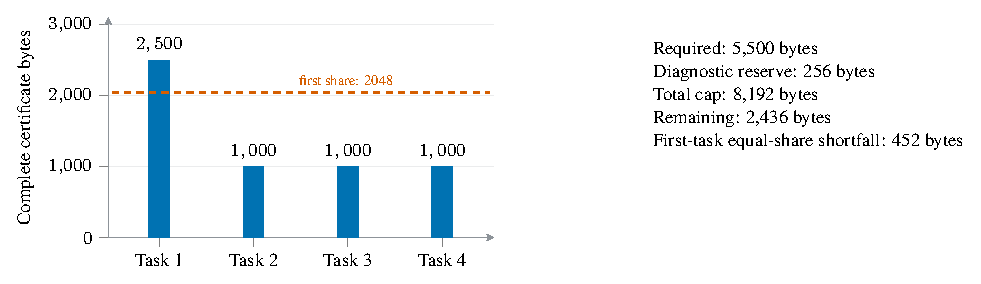
\includegraphics[width=\textwidth]{figures/certificate_budget.pdf}
\caption{完整证书分配的确定性数值反例。单位是实际序列化 UTF-8 bytes，不是 provider tokens；数据来自 A22/A24 受控投递测试。}\label{fig:certificate}
\end{figure}

\begin{pseudocode}{alg:certificate}{原生产者缓存与完整证书投递}
\Pinput{producer ID、不可变完整 bytes、全局池及必需预留}
\Poutput{投递回执或明确预算拒绝}
\Pstep{缓存原 producer 的完整 bytes；相同 ID 但不同 bytes 是协议错误。}
\Pstep{计算本次完整尺寸及其他未投递必需证书预留。}
\Pstep{若无法完整容纳，不发布证明资格；保存私有结果和诊断。}
\Pstep{否则按完整 bytes 计费，生成新的 delivery ID 并保持原 producer ID。}
\Pstep{重投递同一缓存仍扣 bytes；不再次调用生产者，不增加物理执行数。}
\end{pseudocode}
\loc{application/delivery.py; application/service.py}

\subsection{私有观察与原子产物提交}
产品的公共 JSON 与 Markdown 省略源码正文和凭据值；业务 reason 中带标签的秘密在展示时脱敏。文件名、位置和范围仍属于报告信息。原始工具观察及内部异常保存在 \code{.private/observations.jsonl}，文件 0600、目录 0700；内容摘要和引用追溯到原账本。展示脱敏不修改源码身份。

公共 JSON、Markdown 和私有目录在同一 staging 目录准备，原子重命名到尚不存在的最终目录。取消索引或工具阶段时，已登记事实保留，后续工具不再启动。工具内部失败留下私有异常类别与 traceback，而不是丢弃先前充分证据。配置和输出目录本身不能使用时返回结构化 CLI 错误，不覆盖既有目录。

\code{accounting} 分别记录准备、分析、gate、模型及产物准备耗时。JSON 序列化前无法精确知道最终提交总耗时；\code{.private/completion.json} 因而另记包含提交阶段的输出墙钟。默认产品 gate/model 均为零。私有目录权限是本地访问保护，原子提交是产物一致性机制，两者都不构成完整主机隔离证明。\citep{productguide,acceptance}
